\documentclass{ctexart}
\CTEXsetup[format={\Large\bfseries}]{section}            % 让section靠左对齐
\usepackage{graphicx} % Required for inserting images
\usepackage{hyperref}
\usepackage{enumerate} % 下面1,2,3小点


% 设置 subsection 的间距
\usepackage{titlesec}
\titlespacing{\section}{0pt}{0.75\baselineskip}{0.75\baselineskip}
\titlespacing{\subsection}{0pt}{0.5\baselineskip}{0.5\baselineskip}

\usepackage{geometry} % 调整页边距和纸张大小
\geometry{a4paper,scale=0.7} 

\title{\vspace{-2cm}\textbf{程序设计基础课程设计报告} \\ \fontsize{12}{14}{---快速排序算法}}

\author{高宇轩 23009200132}
\date{\today}

\begin{document}
    
    \maketitle
    
    \section{原始题目及要求}
    编写一个程序,对用户输入的若干整数,采用快速排序算法,完成从小到大的排序。
    
    \section{题目分析}
    
    \subsection{题目功能}
    使用快速排序算法,将输入的整数从小到大排序
    \subsection{题目知识点}
    数组、快速排序算法
    
    \section{题目总体方案设计}
    
    \subsection{快速排序算法说明}

    快速排序是一种基于分治策略的排序算法,运行高效,应用广泛。 
    
    快速排序的核心操作是\textbf{“哨兵划分”},其目标是:选择数组中的某个元素作为“基准数”,将所有小于基准数的元素移到其左侧,而大于基准数的元素移到其右侧。
    \newline 
    
    
    快速排序的\textbf{整体流程}如图 1 所示。 
    
    首先,对原数组执行一次“哨兵划分”,得到未排序的左子数组和右子数组。 
    
    然后,对左子数组和右子数组分别递归执行“哨兵划分”。 
    
    持续递归,直至子数组长度为 1 时终止,从而完成整个数组的排序。

    \begin{figure}[h] % 'h' 表示将图片放置在当前位置
        \centering
        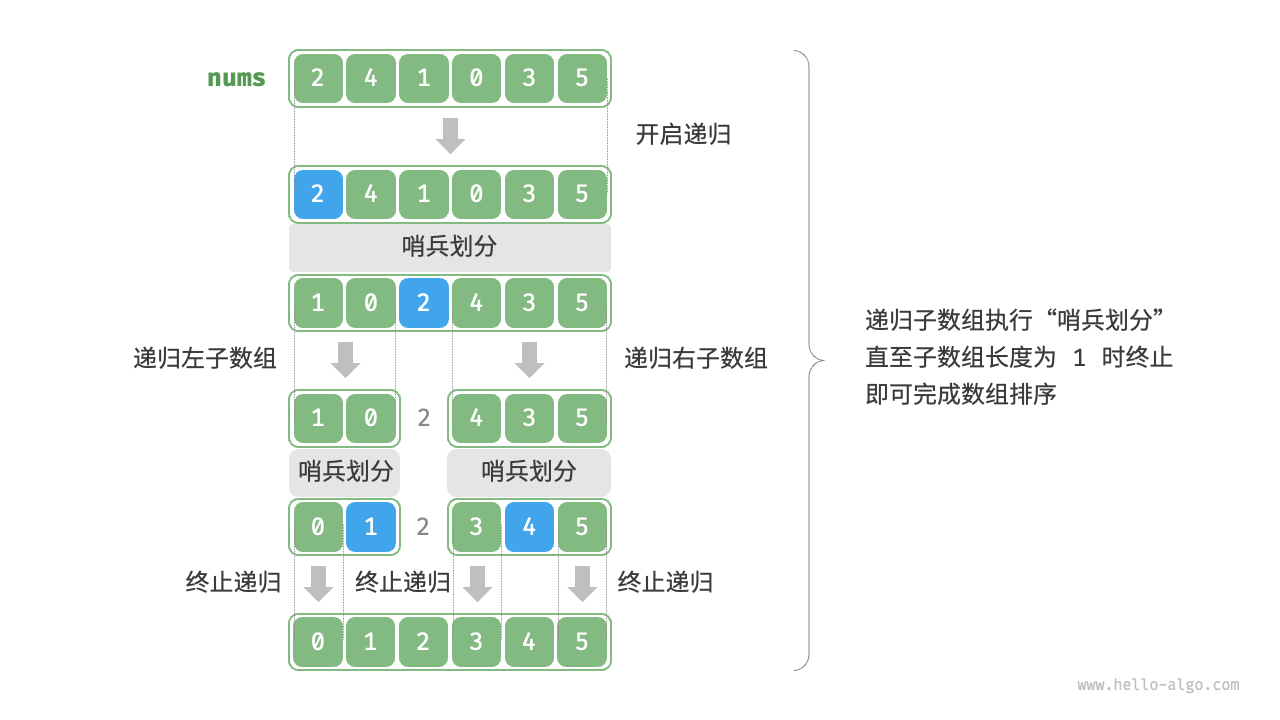
\includegraphics[width=1\textwidth]{algo.png}
        \caption{\href{https://www.hello-algo.com/chapter_sorting/quick_sort/}{快速排序算法示意图}}
    \end{figure}
    \subsection{快速排序中的极端情况}
    快速排序在某些输入下的时间效率可能降低。
    
    当输入数组是完全倒序的,或者数组中的每一个元素都相同时,由于我们选择最左端元素作为基准数,那么在哨兵划分完成后,基准数被交换至数组最右端,导致左子数组长度为 n - 1、右子数组长度为 0 。如此递归下去,每轮哨兵划分后都有一个子数组的长度为 0 ,分治策略失效,快速排序退化为“冒泡排序”的近似形式。
    
    
    \subsection{针对极端情况的优化}
    针对数组完全倒序的情况,我们可以随机挑选一个数为“哨兵划分”中的哨兵,此时特殊情况的算法复杂度会被平摊。
    
    针对数组中每一个元素均相同的情况,我们可以用less,equal,greater三个数组分别存储小于,等于和大于哨兵元素的数组元素,此时只需要对less与greater数组的元素继续递归排序,防止了相同元素导致的算法退化
    
    \section{各功能模块的设计说明}
    在实现quicksort函数时,我们先判断数组元素个数是否小于等于1,作为递归的终止条件,然后用randomPivot函数随机选出一个哨兵元素,用partition函数将划分后的数组放入三个子数组,然后对这三个子数组递归使用quicksort,最后将排序得到的有序数列用catenate函数合并回原来的数组。
    
    randomPivot函数用随机数得到哨兵元素的下标。
    
    partition函数遍历一边原来的数组,将小于、等于、大于哨兵元素的整数分别放入less, equal, greater三个数组中。
    
    catenate函数将三个已经有序的函数分别合并回原来的数组,得到有序的原数组。
    
    \section{程序的集成测试}
    测试程序中,先对我的学号23009200132进行了排序,然后对随机输入的数组进行排序,下面是其中一次运行的结果。
    
     \begin{figure}[h] % 'h' 表示将图片放置在当前位置
       \centering
       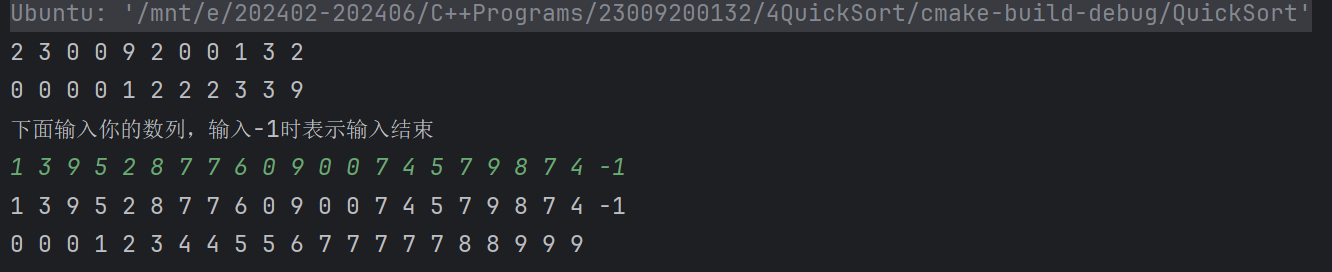
\includegraphics[width=0.8\textwidth]{tests.png}
       \caption{程序的集成测试}   
     \end{figure}
    
    \section{总结}
    实验中用$O(nlogn)$复杂度的快速排序算法实现了整数的排序,同时用随机选择哨兵和三路排序的方式,对快速排序在极端情况下的退化进行了优化。
    
    但是,在算法实现的过程中,为了代码实现的简便,额外使用了大小总计为n的数组,我们还可以用两个指针直接在原数组上对整数进行交换,从而节省空间的使用。
    
    
\end{document}
